\documentclass[tikz,border=8pt]{standalone}
\usepackage{tikz}
\usepackage{xcolor}
\usetikzlibrary{positioning,arrows.meta}
\definecolor{ink}{HTML}{16140F}
\definecolor{cream}{HTML}{F6F4F1}
\definecolor{muted}{HTML}{6D675E}
\definecolor{honey}{HTML}{F0B429}
\begin{document}
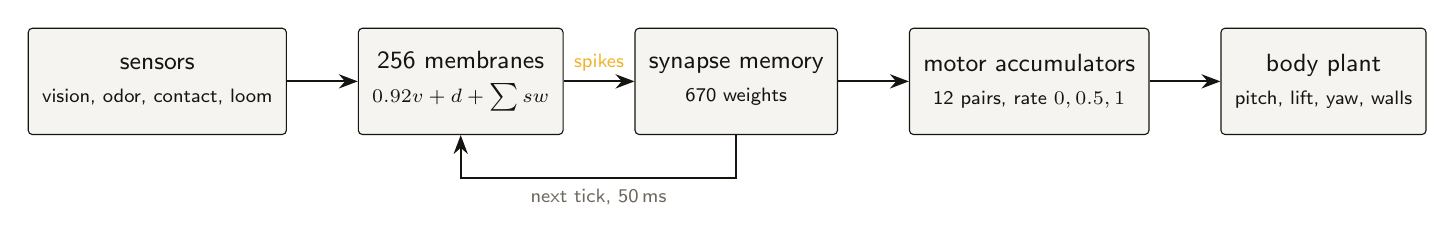
\begin{tikzpicture}[
  font=\sffamily\small,
  block/.style={draw=ink, rounded corners=1.5pt, align=center, minimum height=1.35cm, minimum width=2.55cm, inner sep=5pt, fill=cream, text=ink},
  arr/.style={-{Stealth[length=2.4mm]}, thick, draw=ink},
]
\node[block] (sense) {sensors\\[1pt]\scriptsize vision, odor, contact, loom};
\node[block, right=9mm of sense] (mem) {256 membranes\\[1pt]\scriptsize \(0.92v+d+\sum sw\)};
\node[block, right=9mm of mem] (syn) {synapse memory\\[1pt]\scriptsize 670 weights};
\node[block, right=9mm of syn] (mot) {motor accumulators\\[1pt]\scriptsize 12 pairs, rate \(0,0.5,1\)};
\node[block, right=9mm of mot] (body) {body plant\\[1pt]\scriptsize pitch, lift, yaw, walls};
\draw[arr] (sense) -- (mem);
\draw[arr] (mem) -- node[above, font=\sffamily\scriptsize, text=honey] {spikes} (syn);
\draw[arr] (syn) -- (mot);
\draw[arr] (mot) -- (body);
\draw[arr] (syn.south) -- ++(0,-0.55) -| node[pos=0.25, below, font=\sffamily\scriptsize, text=muted] {next tick, 50\,ms} (mem.south);
\end{tikzpicture}
\end{document}
